\documentclass[twocolumn,pra,showpacs,superscriptaddress,longbibliography]{revtex4-1}   % use preprint or twocolumn
\usepackage{graphicx}
\usepackage{amsmath}
\usepackage{amssymb}
\usepackage{epstopdf}
\usepackage{dcolumn}% Align table columns on decimal point
\usepackage{bm}% bold math
\usepackage{verbatim}
\usepackage{amsfonts}
\usepackage{cancel}
\usepackage[utf8]{inputenc}
\usepackage{graphicx}
\usepackage{setspace}
\usepackage{tabularx}
\usepackage[export]{adjustbox}



\DeclareGraphicsRule{.tif}{png}{.png}{`convert #1 `dirname #1`/`basename #1 .tif`.png}


\newcommand{\sspace}{$\enspace$}
\newcommand{\ssspace}{$\quad$}
\newcommand{\proofend}{\mbox{ }\hfill$\Box$\\}
\newcommand{\deriv}[2]{\frac{\mathrm{d} #1}{\mathrm{d} #2}}
\newcommand{\parderiv}[2]{\frac{\partial #1}{\partial #2}}
\newcommand{\ee}[1]{\cdot 10^{ #1}}
\newcommand{\bra}[1]{\left\langle #1 \right|}
\newcommand{\ket}[1]{\left| #1 \right\rangle}
\newcommand{\braopket}[3]{\left.\left\langle #1 \right|\right|#2\left|\left| #3 \right\rangle\right.}
\newcommand{\dbbraopket}[3]{\left.\left\langle#1\right.\right.\|#2\|\left.\left.#3\right\rangle\right.}
\newcommand{\braket}[2]{\left\langle #1 \right|\left. #2 \right\rangle}
\newcommand{\trace}[1]{\mathrm{Tr}\left(#1\right)}
\newcommand{\abs}[1]{\left|#1\right|}
\newcommand{\avg}[1]{\left\langle #1 \right\rangle}
\newcommand{\figref}[1]{Fig.~\ref{#1}}
\newcommand{\eqnref}[1]{Eqn.~\eqref{#1}}


\newcommand{\AAA}{\mathrm{\AA}}

\newcommand{\abinit}{\textit{ab initio}}
\newcommand{\abinitspace}{\textit{ab initio} }




\begin{document}

\title{Notes on calculating atom interferometer gyroscope sensitivity}
\maketitle


\subsection{Theory}

The goal of this project is to allow us to explore how the sensitivity of a Mach-Zehnder atom interferometer gyroscope is determined by:
\begin{itemize}
	\item choice of atom (and its associated van der Waals $C_3$ coefficient)
	\item atom velocity $v$
	\item grating period $d_g$
	\item grating open fraction (defined as $w/d_g$, where $w$ is the width of the gaps between adjacent grating bars)
	\item grating longitudinal thickness $l$
	\item longitudinal distance between successive gratings $L$
\end{itemize}
Choosing the grating thickness $l$ and grating-to-grating distance $L$ is likely fairly simple: we always want smaller $l$ and larger $L$, but $l$ will probably be determined by the grating fabrication process and $L$ is limited by the maximum size of the apparatus. The grating period $d_g$ and open fraction $w/d_g$ can be optimized for a choice of atom and atom velocity $v$. Therefore, we want to be able to plot the sensitivity of a Mach-Zehnder atom interferometer gyroscope as a function of $v$ for different atoms.

The sensitivity $S$ of a gyroscope is described as 
\begin{align}
	S = \delta\Omega \sqrt{t}
	\label{sensitivityGeneral}
\end{align}
where $\delta\Omega$ is the uncertainty in a typical measurement of rotation rate $\Omega$ and $t$ is the amount of data acquisition time required to make that measurement. 
Smaller values of $S$ are preferable.
Values of $S$ are usually expressed in $rad/s/\sqrt{Hz}$. 
$S$ also is a measure of the uncertainty in the gyroscope's angular orientation as a function of operating time and is therefore sometimes expressed in $^{\circ}/\sqrt{h}$ (i.e. the uncertainty in the gyroscope's angular orientation is $S\sqrt{T}$, where $T$ is the operating time since last calibration).

This sensitivity $S$ can be written in terms of the items listed previously.
For an atom interferometer gyroscope, the phase $\phi$ can be written as
\begin{align}
	\phi = \frac{4\pi\vec{\Omega}\cdot\vec{A}}{\lambda_{dB} v} - \phi_0
\end{align}
where $\phi_0$ is an arbitrary refrence phase, $\lambda_{dB}$ is the atoms' de Broglie wavelength, and $\vec{\Omega}\cdot\vec{A}$ is the projection of the gyroscope's rotation rate vector $\vec{\Omega}$ onto the plane of the interferometer with enclosed area $A$. If we let $\Omega$ be the component of $\vec{\Omega}$ normal to $\vec{A}$ and represent $\lambda_{dB}$ as $h/mv$, we can rewrite the above equation as
\begin{align}
	\delta\phi = \frac{4\pi m A}{h}\delta\Omega
\end{align}
and solve it for $\delta\Omega$ to get
\begin{align}
	\delta\Omega = \frac{h}{4\pi m A}\delta\phi
	\label{deltaOmega}
\end{align}

According to \cite{Lenef1997}, the uncertainty $\delta\phi$ on a single measurement of the phase of an atom interferometer is defined by
\begin{align}
	\delta\phi^2 = \frac{1}{|C|^2N}
	\label{phaseSDev}
\end{align}
where $N$ is the number of atoms detected.
Substituting Eq. \ref{phaseSDev} into Eq. \ref{deltaOmega} and the result into Eq. \ref{sensitivityGeneral}, we get 
\begin{align}
	S = \frac{h}{4\pi m A} \sqrt{\frac{t}{|C|^2N}}
	\label{sensitivity2}
\end{align}
If we take $t$ to be the unit time, we see $N/t$ is the average atom beam intensity (i.e. flux) $\avg{I}$.

The interferometer's enclosed area $A$ can be written as
\begin{align}
	A = L^2\tan{\theta_d} = L^2\tan\left(\arcsin\left(\frac{h}{mvd_g}\right)\right) \approx \frac{L^2h}{mvd_g}
\end{align}
Substituting into Eq. \ref{sensitivity2}, we get
\begin{align}
	S = \frac{vd_g}{4\pi L^2} \frac{1}{ \sqrt{|C|^2\avg{I}}}
	\label{sensitivity3}
\end{align}


\cite{Cronin2005} describes in detail how to calculate $|C|^2\avg{I}$ from the nanograting open fraction, thickness, and period as well as atom velocity and atom-grating $C_3$ coefficient. This calculation can be done with and without considering van der Waals interactions between the atoms and the grating bars. 
Kapitza-Dirac gratings can be represented as gratings for which $C_3 = 0$ and the open fraction $f = 1/2$.

Note that the $\left(e_n^{Gi}\right)^2$ terms in Eq. 14 in \cite{Cronin2005} should actually be written as $\left|e_n^{Gi}\right|^2$.

van der Waals $C_3$ coefficients for alkali metals interacting with various media (including silicon nitride) are listed in atomic units in \cite{Arora2014}. To convert the $C_3$ coefficients in atomic units to SI units (for the sake of the numerical calculations), multiply by 1 Hartree times the Bohr radius cubed. Useful $C_3$ coefficients are listed in SI units in Table \ref{tableC3}.

\begingroup
\begin{table}
\caption{\label{tableC3} van der Waals $C_3$ coefficients in units of $10^{-49}$ Jm$^3$ for various combinations of atoms and dielectric media \cite{Arora2014}.}
\begin{center}
\begin{tabular}{l|ll}
\hline\hline
& SiN$_x$ & SiO$_2$ \\
\hline
Li & 4.61 & 3.10 \\
Na & 5.10 & 3.49 \\
K &  7.82 & 5.42 \\
Rb & 8.85 & 6.20 \\
\hline\hline
\end{tabular}
\end{center}
\end{table}
\endgroup


\subsection{Results}

\begin{figure*}
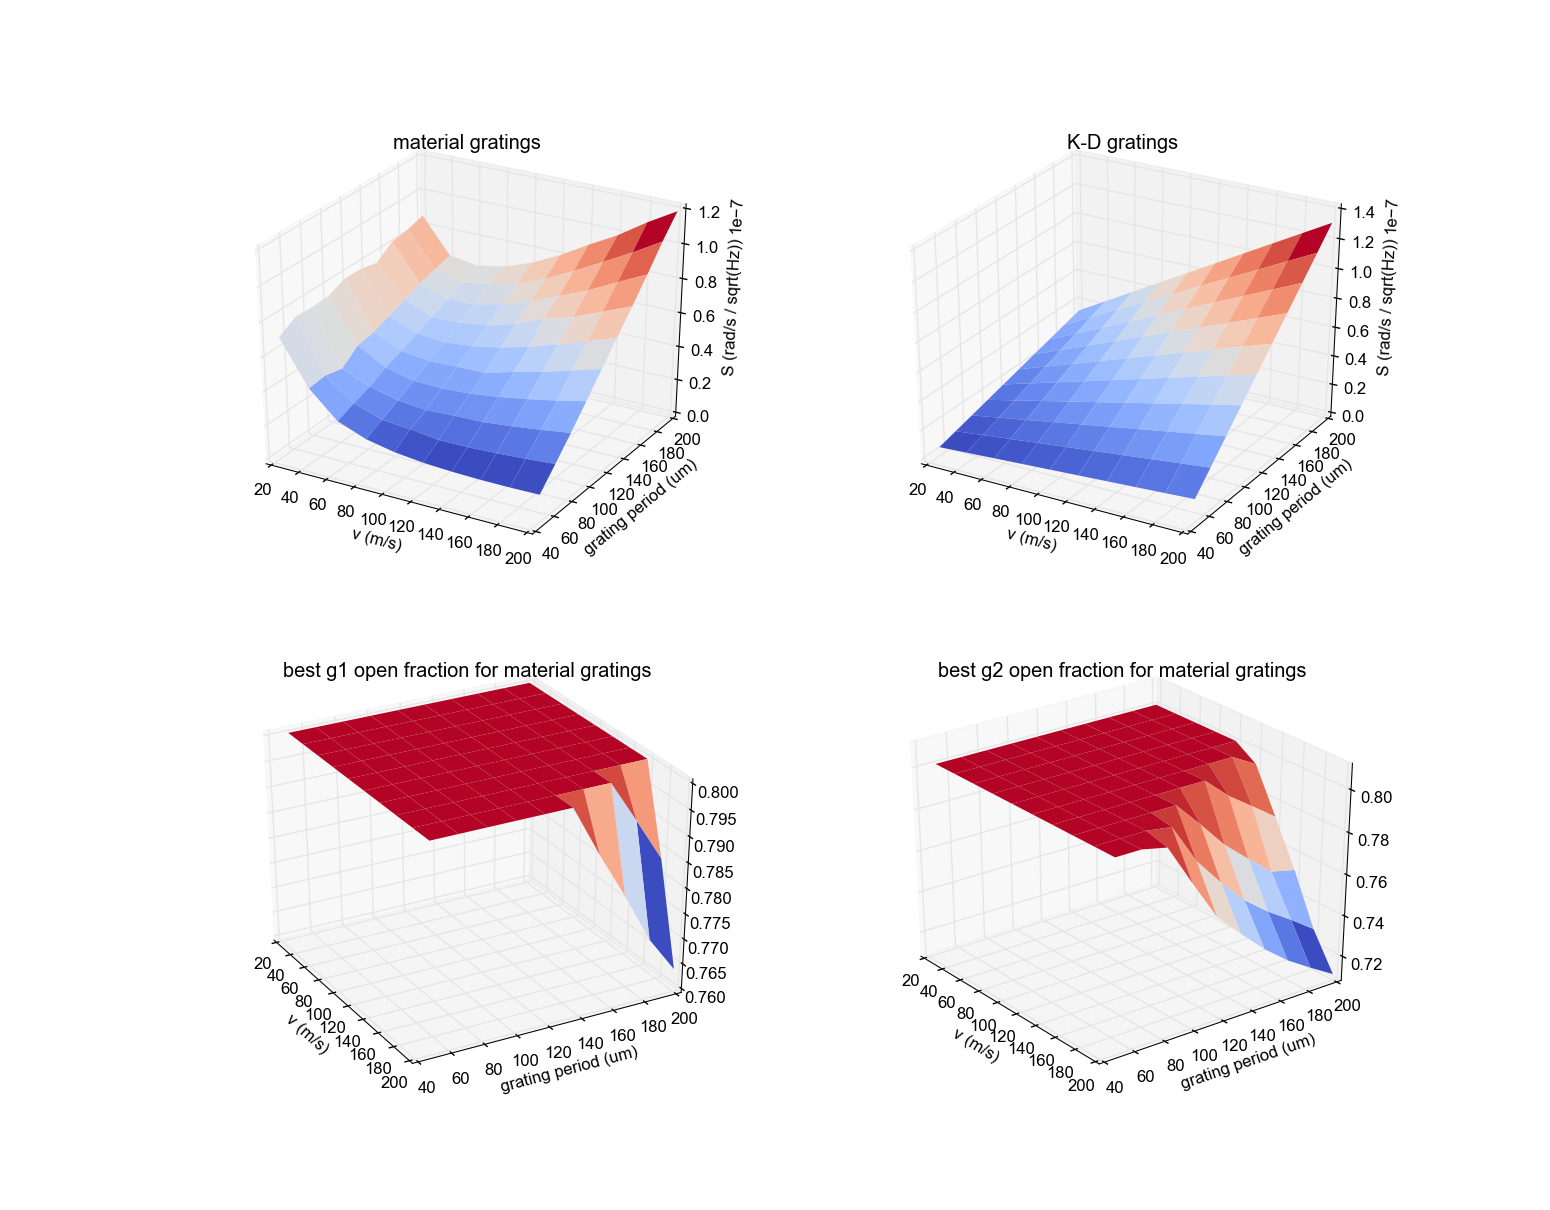
\includegraphics[width=\linewidth,keepaspectratio]{../plots/Sf1f2_vs_dv_Rb_L10cm.png}
\caption{\label{S_vs_dv} TOP LEFT: Sensitivity $S$ of an atom interferometer gyroscope as a function of atom velocity $v$ and grating period $d$. For this calculation, it was assumed that $L = 10$ cm and the $C_3$ coefficient was that of Rb interacting with SiN$_x$. TOP RIGHT: Same as top left, but for Kapitza-Dirac gratings (open fractions set to 1/2, $C_3 = 0$). BOTTOM LEFT and BOTTOM RIGHT: optimal open fractions for gratings 1 and 2 as a function of $v$ and $d$. The optimal open fractions were capped at 0.8, since there is a physical limit to how small the grating bars can be. 0.8 was simply a guess at this limit--the actual limit likely depends on $d$.}
\end{figure*}

Fig \ref{S_vs_dv}, top left, shows the sensitivity of an atom interferometer gyroscope with material gratings as a function of $v$ and $d$. For this calculation, it was assumed that $L = 10$ cm and the $C_3$ coefficient was that of Rb interacting with SiN$_x$. This figure indicates that sensitivity $S$ always improves as grating period decreases and that the optimal velocity $v$ increases as $d$ decreases. 




\bibliography{library}

\end{document}  